
\section{Numerical approach}
\subsection{Introduction: the non-hydrostatic correction}
%kurze Hinführung, was muss diskretisiert werden, fractional step, rolle der korrekturformeln, algorithmus, integralform?
In the following, a short summary of the non-hydrostatic correction shall be presented. For a more self-contained and detailed discussion, please refer to  \cite{samfass14extension}, \cite{cui} and \cite{fuchs}. 

The basis for the method presented in this paper are the non-hydrostatic shallow water equations as given by:
\begin{align}
\boxed{
{\begin{bmatrix}
h \\
hU\\
hV\\
hW
\end{bmatrix}}_{t}
+
{\begin{bmatrix}
hU \\
hU^2+\frac{1}{2}gh^2\\
hUV\\
hUW
\end{bmatrix}}_{x}
+
{\begin{bmatrix}
hV \\
hUV\\
hV^2+\frac{1}{2}gh^2\\
hVW
\end{bmatrix}}_{y}
=
{\begin{bmatrix}
0 \\
-ghb_x -\left([ \frac{hq}{2}]_x+[q]_{z=b}b_x \right)\\
-ghb_y -\left([ \frac{hq}{2}]_y+[q]_{z=b}b_y \right)\\
[q]_{z=b}
\end{bmatrix}_.}}
\label{eq:govern}
\end{align}

Here, $h (x,y)=\eta (x,y) -b(x,y)$ denotes the height of the water column, $\eta (x,y)$ the free surface elevation above the mean sea level, $b (x,y)$ the bathymetry, $(U,V,W)$ the depth-averaged velocity vector, $g$ the gravity of Earth and a subscript the partial derivative with respect to the given coordinate. Further, $q (x,y,z)$ represents the non-hydrostatic portion of the pressure. Note that $q$ will not be the real non-hydrostatic pressure but only a numerical correction parameter. This term stems from the pressure decomposition
\begin{equation}
p= p_H + q = g (\eta -z) +q
\end{equation}
into a hydrostatic portion $p_H$ and a non-hydrostatic part $q$ as suggested in \cite{casu} which has been used in the depth-integration of the Navier Stokes equations. In the hydrostatic shallow water equations, $p=p_H$ is assumed instead. Stated differently, the hydrostatic shallow water equations are received as a special case of \eqref{eq:govern} by setting $q=0$. 

The non-hydrostatic shallow water equations \eqref{eq:govern} involve certain assumptions which are reviewed subsequently. We follow \cite{walters} and assume a linear vertical distribution of the non-hydrostatic pressure. Thus, for the depth-averaged non-hydrostatic pressure occuring during the depth-integration,
\begin{equation}
\frac{1}{h} \int_{b}^{\eta} q \, dz= \frac{1}{2} [q]_{z=b}
\end{equation}
holds since the non-hydrostatic pressure vanishes at the surface. In addition, the vertical velocity component $w$ is approximated linearly in z-direction \cite{walters}. Hence, with the assumption of a zero vertical velocity at the bottom (cf. \cite{cui}):
\begin{equation}
W=  \frac{1}{h} \int_{b}^{\eta} w \, dz= \frac{1}{2} [w]_{z=\eta}.
\end{equation}
Thus, only the vertical velocity at the water surface will be computed in the model. We therefore drop the subscript for simplicity in the remainder of this paper.

In order to solve the non-hydrostatic shallow water equations \eqref{eq:govern} with these assumptions, we employ the commonly applied implicit fractional step scheme: in each time step, the hydrostatic shallow water equations are solved with the finite volume method first. After the hydrostatic solution has been computed, the discharges $hU$ and $hV$ and the vertical velocity $w$ at the surface will be corrected with the non-hydrostatic pressure $[q]_{z=b}:=\hat q$ at the bottom. This numerical parameter will be obtained by a pressure projection as introduced in \cite{chorin}: it is computed as the solution to a system of linear equations in order to render each numerical control volume divergence-free. Naturally, the basis for the derivation of the system of linear equations will therefore be the law of mass-conservation of the Navier-Stokes equations:
\begin{equation}
\frac{\partial u}{\partial x}
+
\frac{\partial v}{\partial y}
+
\frac{\partial w}{\partial z}
=
0.
\label{eq:mass_consv}
\end{equation}

In order to derive the system of Poisson equations for the non-hydrostatic pressure, correction formulas will be plugged into the integral form of \eqref{eq:mass_consv} and discretized in space, see Sec. TODO. These formulas express how the discharges/velocities have to be corrected with the non-hydrostatic pressure and follow from a first-order Euler time-discretization of the governing equations \eqref{eq:govern}:
\begin{align}
(hU)^{n+1}&= (\widetilde{hU})^{n+1} -\Delta t \left(\left[\frac{1}{2}h^{n}\hat{q}^{n+1}\right]_x+\hat q^{n+1}b_x\right)
\\
(hV)^{n+1}&= (\widetilde{hV})^{n+1} -\Delta t \left(\left[\frac{1}{2}h^{n}\hat{q}^{n+1}\right]_y+\hat q^{n+1}b_y\right)
\\
w^{n+1}&= \widetilde{w^{n+1}}+ 2\Delta t \frac{\hat q^{n+1}}{h^{n+1}}.
\end{align}
Here, the tilde is used to represent the intermediate quantities computed by the hydrostatic solver in each time-step. Note that for the vertical velocity correction formula, the vertical momentum equation in  \eqref{eq:govern} has been divided by $h$ and the non-linear terms have been neglected (cf. \cite{cui}). Because of the latter approximation, the hydrostatic solver does not have an impact on the vertical velocity ($\widetilde{w^{n+1}}=w^{n}$). 



%For a detailed derivation, various sources are available, refer e.g. to \cite{samfass14extension}, \cite{cui} or \cite{fuchs}.  


\subsection{Discretization on Triangular Grids in \samoa}

\subsubsection*{Introduction to \samoa}
Before the spatial discretization of the non-hydrostatic pressure equation can be explained, some preliminary remarks on the simulation package \samoa and its numerical model for solving the hydrostatic shallow water equations have to be made.

\samoa is a parallel framework for solving partial differential equations on dynamically adaptive triangular meshes. It uses the Sierpinski space-filling curve in order to provide memory and cache-efficient algorithms for grid generation, refinement and traversal and supports finite element, finite volume and discontinuous-Galerkin discretizations \cite{meister11software}.  

In this paper, we focus only on the SWE subpackage in \samoa which implements the finite volume method for solving the 2D-hydrostatic shallow water equations based on the theory in \cite{leveque}. For each finite volume cell $i$, a cell average or state $Q_i^{n}= (h_i^{n},[hU]_i^{n},[hV]_i^{n})^T$ is determined. In order to compute $Q_i^{n+1}$ during a timestep, each $Q_i^{n}$ is updated with the numerical fluxes which are computed by solving Riemann problems on the cell edges. The timestep $dt$ is restricted by the CFL-condition and thus varies depending on the scenario and the grid resolution.  

Regarding the grid generation, \samoa starts with a square that is divided by its diagonal into two right triangles/cells as its computation domain. Initially, these two triangles are then refined recursively into smaller right triangles through bisection until a sufficient grid resolution is obtained (cf. \ref{fig:adapt_grid}). Cells can also be refined during the simulation in an analogous manner. The state of new cells generated in this process is determined using a simple interpolation according to the (constant) basis functions. On the other hand, the reverse process (i.e. coarsening) might happen as well: two right triangles of the same refinement depth are merged into a single one by computing an average of the two cell states.

A key element used in \samoa is the grid traversal through which access to the grid variables is granted. During such an traversal, different operators are called such as the element operator ELEMENT\_OP which is being called for each element. The NODE\_FIRST\_TOUCH\_OP and NODE\_LAST\_TOUCH\_OP operators allow for a different treatment of a node depending on whether the node is visited for the first or for the last time in a traversal.

\begin{figure}
\centering
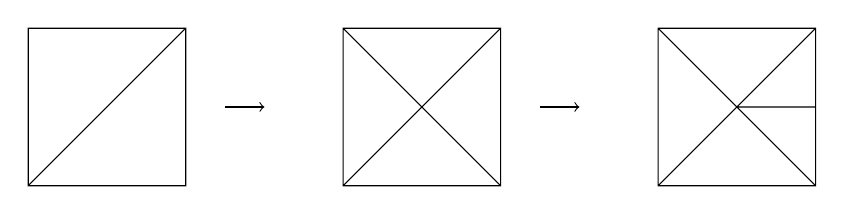
\begin{tikzpicture}
\draw (0,0) rectangle (2,2) -- (0,0);
\draw[->] (2.5,1) -- +(0.5,0);
\draw (4,0) rectangle ++(2,2) -- (4,0) ++(0,2) -- ++(2,-2);
\draw[->] (6.5,1) -- +(0.5,0);
\draw (8,0) rectangle ++(2,2) -- (8,0) ++(0,2) -- ++(2,-2) ++(0,1) -- +(-1,0);
\end{tikzpicture}
\caption{Example refinement: in the first step, both cells are refined while in the second, only the rightmost cell is refined.}
\label{fig:adapt_grid}
\end{figure}

\subsubsection*{Dual Grid Discretization}
The non-hydrostatic extension as reviewed previously introduces two additional degrees of freedom: the vertical velocity $w$ at the water surface and the non-hydrostatic pressure correction parameter $\hat q$ at the bottom. In \cite{samfass14extension}, these quantities were co-located with the other variables $h,hU,hV$ in the centers of the rectangular cells. The non-hydrostatic correction formulas were discretized using finite differences to obtain the system of linear equations for $\hat q$. However, the realization of this approach is not directly applicable in \samoa. First, the adaptivity of the grid would be problematic for determining the mesh-width of the differences which would be necessary in order to compute the non-hydrostatic pressure gradients. Second, accessing neighbouring cell data would be required for the assembly of the global matrix for the non-hydrostatic pressure. However, the underlying traversal concept of \samoa does not allow this. 

In order to circumvent these difficulties, we propose to use a dual grid for the control volumes for the non-hydrostatic pressure. 

%initial attempts: finite differences -> problems with number of unknowns, discontinuity
%picture with examples for assembly of the equations, matrix-free jacobi
%derivation of the element matrix, reference element
%boundary conditions: neumann and dirichlet
%rotation pressure gradients/normals
%computation of the boundary integrals
%interpolation of w (vs. averaging) and q on the nodes->adaptivity
%reduction to poisson equation, stencil, pseudo-symmetry